\documentclass[a4paper]{article}

\usepackage[utf8]{inputenc}

\usepackage{url}
\usepackage[]{hyperref}

\usepackage{caption}

\usepackage{listings}

\usepackage{color}
\usepackage[table]{xcolor}

% *** GRAPHICS RELATED PACKAGES ***
%\usepackage[pdftex]{graphicx}
\usepackage{graphicx}
%\usepackage[dvips]{graphicx}
% to place figures on a fixed position
\usepackage{float}

\usepackage{amsmath}

\usepackage[margin=1in]{geometry}


\title{Evaluation of High-speed transport protocol simulations}
\author{Sonkoly, Balázs (transport protocols) \\ Németh,Felicián (Network Simulator) \\Császár András (Network
Simulator) \\ Janky, Ferenc (English translation)
}
\date{}


\begin{document}

\maketitle

\tableofcontents

\section{Introduction}

\textbf{Transmission Control Protocol (TCP)} has been used for congestion control in the Internet for decades. During
the evolution of the Internet a lot have been changed about the traffic patterns of applications and also in the
structure of the networks. Wireless and high-speed network environments pose new challenges that can be tackled by
current TCP version only at the price of many trade-offs.

TCP -- one of the most important transport protocol of the Internet -- has a history of many decades. The initial
protocol -- that was called \emph{Network Control Protocol - NCP} -- is originated from the '70s. Out of this protocol
had emerged the TCP/IP network's two foundational protocols: IP operating in the network level, and
TCP~\cite{CongestionAvoidance} operating in the transport level. TCP has many features that are required for proving
reliable transport services. Congestion control is one of its main feature that protects the network from
over-utilization. The connection-oriented TCP protocol does closed-loop control during which the transmitter adjusts
its transmission speed based on the incoming acknowledgments affected by the network conditions aimed for having
optimal network utilization and to avoid network breakdown by over-utilization. The initial version was finalized in
\href{http://www.faqs.org/rfcs/rfc793.html}{RFC 793} in 1981. The base mechanism had been extended gradually with new
methods like \textbf{Slow Start}, \textbf{Congestion Avoidance}, RTO calculation, delayed acknowledgment in
1989(\href{http://www.faqs.org/rfcs/rfc1122.html}{RFC 1122}), selective acknowledgment (\textbf{SACK}) in 1996
(\href{http://www.faqs.org/rfcs/rfc2018.html}{RFC 2018}) or definition of \textbf{NewReno} version in 2004
(\href{http://www.faqs.org/rfcs/rfc3782.html}{RFC 3782}).

\section{Conventional TCP: TCP Reno}

TCP's main task is implement congestion control in a distributed, closed-loop system in a way that the users can
utilize the available network bandwidth in an optimal and fair manner. The latter attribute is commonly referred as a
protocol's \textbf{fairness} that is going to be a main aspect in future network's beside efficiency. In case of new
protocols and new control mechanisms -- in contrast with traditional TCP's traditional design methodology -- the
findings and theory of control theory and optimization theory can be utilized during the design phase.

During a TCP connection the transmitting party sends data packets over the network and the receiving side provides
cumulative acknowledgments that informs the sending side about the so far correctly received packets. The TCP
transmitter can send a new packet in case of a received acknowledgment that realizes a from of closed-loop control
(\textbf{self-clocking}). In TCP the congestion control is realized using a sliding-window mechanism where the
transmitter can only have a number of outstanding unacknowledged packets in the network corresponding to the size of
the \textbf{congestion window (cwnd)}. The size of the congestion window is a state variable (beside many others)
controlled by the transmitter entity that can be used for controlling the transmission speed. The main task of the
congestion control algorithm is to control this state variable as a function of the network conditions. TCP Reno
controls this \emph{cwnd} variable differently in different phases of the connection. After connection establishment --
when the network conditions are yet unknown on the network path -- the control of the cwnd and the speed happens using
the \textbf{Slow Start} algorithm. In this phase -- despite the name of the algorithm -- the congestion window expands
exponentially until it reaches a threshold or packet loss occurs. After one of these events the long term behavior is
determined by the \textbf{Congestion Avoidance} phase when the protocol tries to control the transmission speed so that
it won't cause severe congestion in the network. In this phase the congestion window is controlled by the \textbf{AIMD}
(Additive Increase Multiplicative Decrease) mechanism. As a result of this control the congestion window takes on a
typical oscillating, sawtooth pattern.

There are two more mechanisms worth noting here that performs correction of lost packets. These are the \textbf{Fast
    Retransmit} and \textbf{Fast Recovery}. When TCP reno detects multiple ACKs for the same packet (that means the
receiver still expects to receive the same packet) then it implies a packet loss event with not significant congestion
since the subsequent packets have reached the receiver successfully. After 3 duplicate ACKs it retransmits immediately
the missing packet (Fast Retransmit) and transfers into Fast Recovery phase. The transmission does not cease in Fast
Recovery phase, the transmitter can send new packets into the network based on the current value of cwnd and the
received ACKs. As soon as the missing packet has been ACK-ed TCP Reno goes back into Congestion Avoidance. The protocol
differentiates the packet loss due to extreme congestion using a timer that is started after sending each packet. If
this timer expires (RTO, Retransmission Time Out) that means ACKs from the receivers are completely missing or too many
packets have been lost. In such case TCP Reno implies extreme network congestion and restarts in Slow Start. The
different phases of TCP Reno are illustrated on Figure~\ref{fig:TCP-Reno-operation}. Further details can be found
in~\cite{CongestionAvoidance} (can be downloaded from
\href{http://qosip.tmit.bme.hu/cgi-bin/twiki/viewfile/VITT5318/WebHome?rev=1;filename=jacobson88congestion.pdf}{here}).

\begin{figure}[H]
    \centering
    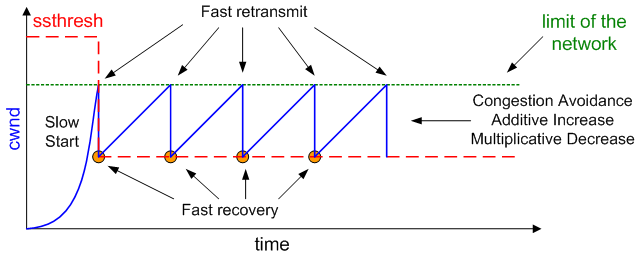
\includegraphics[width=0.9\textwidth]{figures/tcp-reno.png}
    \caption{The operation and phases of TCP Reno}
    \label{fig:TCP-Reno-operation}
\end{figure}

The properties of AIMD algorithm ensures that the TCP Reno flows transmission speed converges to the fair state in case
of the flows have identical round trip time (RTT). This operation is illustrated by Figure~\ref{fig:AIMD}. Out of the
linear control methods AIMD is capable to provide the convergence to the optimal state from any point in this state
space for providing maximum utilization and fairness. Think about why not MIMD, AIAD and MIAD mechanism are not
convergent!

\begin{figure}[H]
    \centering
    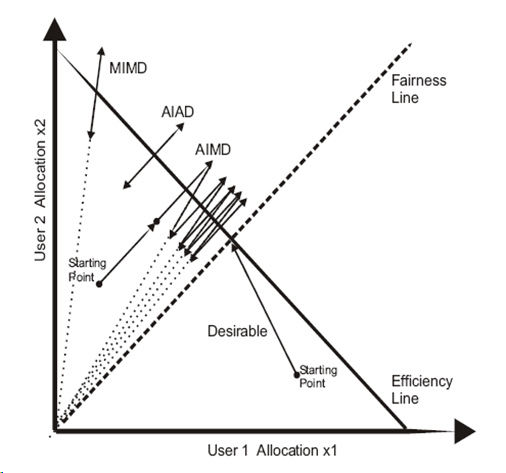
\includegraphics[width=0.9\textwidth]{figures/AIMD-trajectory.png}
    \caption{AIMD trajectory in case of two flows with equivalent RTT }
    \label{fig:AIMD}
\end{figure}

The sawtooth pattern originated from the AIMD can be examined on Figure~\ref{fig:sawtooth}. It's clearly visible that
in case of no packet-loss the cwnd grows linearly (additive increase) and when a packet loss occurs the cwnd halves
(multiplicative decrease). This operation is implemented by increasing cwnd by \textbf{cwnd} for each received ACK that
roughly translates to increase by 1 under one RTT. In case of detecting a packet loss the cwnd is halved. The essence
of the method in mathematical format is the following:

\begin{tabular}{ll}
    per-ACK: & $\texttt{cwnd} \leftarrow \texttt{cwnd} + \dfrac{1}{\texttt{cwnd}}$  \\
    per-RTT: & $\texttt{cwnd} \leftarrow \texttt{cwnd} + 1$                         \\
    loss:    & $\texttt{cwnd} \leftarrow \texttt{cwnd} - \dfrac{\texttt{cwnd}}{2}$  \\
\end{tabular}

\begin{figure}[H]
    \centering
    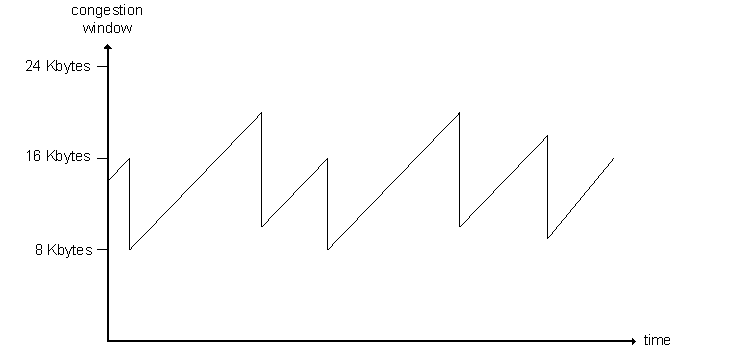
\includegraphics[width=0.9\textwidth]{figures/sawtooth.png}
    \caption{Sawtooth plot}
    \label{fig:sawtooth}
\end{figure}

The basic TCP reno mechanism is not efficient if multiple packets are lost under one round trip (packet loss burst)
because this can not be corrected efficiently by the Fast Retransmit/Fast Recovery mechanism. For fixing this issue
Selective Acknowledgment had been added (SACK) that can be used by the receiver to inform the transmitter in detail on
which blocks of the packet sequence has been received and which are missing. This naturally involves modifying the
implementation of both the sender and receiver TCP entity. Furthermore the TCP header is extended with a corresponding
optional block (SACK option header). Nowadays most TCP implementations provide the SACK extension.

\section{Congestion control principles}

It has been shown that for TCP Reno the indicator for congestion is a packet loss event that occurs when the queues
overflow on a link with the smallest bandwidth (i.e. the bottleneck link). This method -- called \textbf{packet loss
    based} congestion control -- is present in several new, high-speed TCP version however it has some drawbacks as
well.
The actual congestion control is can be carried in 1 bit of information (packet loss/no packet loss) as a consequence
it does not allow fine-grained or sophisticated control algorithms to be used. Furthermore packet-loss based control
involves filling up queues since the control action is only carried out in case of a packet loss. That infers the
presence of oscillation that incurs  system wide stability issues. Another control approach is to measure the RTT of
individual packets and control the transmission speed based on this input. These \textbf{delay-based} methods aims for
a single TCP flow keeping a given amount of packets in the network queues along the network path. These protocols
estimate the components of RTT using a certain method. The components are the physical propagation time and the queuing
time. In these type of algorithms the latter one is subject to be controlled by different methods.
The newest methods combine the packet loss and delay-based methods into a \textbf{hybrid} algorithm for congestion
control where the transmitter reacts to both packet loss and change in delay events. Even more sophisticated methods
are applied by some protocols that utilize \textbf{passive or active measurement methods} for estimating the available
network bandwidth and performing control.

In the previously described methods the transmitter has the necessary logic  and the concrete algorithms can be
improved flexibly or even replaced completely without changing other parts of the network. However there is a concept
that the current state of the network congestion is reported by the network routers explicitly to the transmitter.
These \textbf{explicit congestion signaling} methods requires modification of existing network routers.

\section{High-Speed TCP versions}
\begin{table}
    \begin{tabular}{|p{0.25\textwidth}|p{0.25\textwidth}|p{0.25\textwidth}|p{0.25\textwidth}|}\hline
        \cellcolor{blue!25}protocol                                                   & \cellcolor{blue!25}type
                                                                                      & \cellcolor{blue!25}suggested
        by,when                                                                       &
        \cellcolor{blue!25}properties
        \\\hline
        \cellcolor{blue!25}HighSpeed TCP                                              & packet loss based
                                                                                      & S. Floyd, International
        Computer Science Institute (ICSI),
        Berkeley University of California, 2003.                                      & AIMD
        \\\hline
        \cellcolor{blue!25}Scalable TCP                                               & packet loss based
                                                                                      & T. Kelly, CERN \& University of
        Cambridge, 2003.                                                              & MIMD
        \\\hline
        \cellcolor{blue!25}BIC TCP/CUBIC                                              & packet loss based
                                                                                      & I. Rhee et al., Networking
        Research Lab, North Carolina State
        University, 2004-2005.                                                        & Good utilization,fairness \&
        stability
        \\\hline
        \cellcolor{blue!25}FAST TCP                                                   & delay-based
                                                                                      & S. Low et al., Netlab,
        California Institute of Technology, 2004. (now:
        FastSoft Inc.)                                                                & promising fairness properties
        \\\hline
        \cellcolor{blue!25}TCP Westwood                                               & measurement based
                                                                                      & M.Y. Sanadidi, M. Gerla et al.,
        High Performance Internet Lab,
        Network Research Lab, University of California, Los Angeles (UCLA), 2001-2005 & multiple variants, different
        approximation methods
        \\\hline
        \cellcolor{blue!25}Compound TCP                                               & hybrid
                                                                                      & K. Tan et al., Microsoft
        Research, 2005.                                                               & AIMD + delay-based
        component
        \\\hline
        \cellcolor{blue!25}XCP                                                        & explicit congestion signaling
                                                                                      & D. Katabi et al., Massachusetts
        Institute of Technology (MIT),
        2002.                                                                         & change in network routers
        required
        \\\hline
    \end{tabular}
    \caption{Overview High-Speed TCP versions}
    \label{table:tcpver}
\end{table}

In the following there will be brief overview of the more important protocols and their potential future role.
Table~\ref{table:tcpver} has a compact summary on this topic while a more detailed version can be found
in~\cite{TCPFairnessAnalysis}. Firstly the more significant packet loss based variants are introduced. One of the first
high-speed TCP version was \textbf{HighSpeed TCP}~\cite{HighSpeedTCP} that uses AIMD with a simple modification. This
protocol becomes more adaptive because it changes the conventionally static parameters of AIMD dynamically based on the
size of the congestion window. This results in more aggressive increase of cwnd in large-scale high-speed networks
while also resulting in milder throttling. The concrete operation can be formalized as:

\begin{tabular}{ll}
    per-ACK: & $\texttt{cwnd} \leftarrow \texttt{cwnd} + \dfrac{a(\texttt{cwnd})}{\texttt{cwnd}}$  \\
    loss:    & $\texttt{cwnd} \leftarrow \texttt{cwnd} - b(\texttt{cwnd})\texttt{cwnd}$            \\
\end{tabular}

It can be shown that this is a generalization of TCP Reno with $\texttt{a(cwnd)}=1$ and $\texttt{b(cwnd)}=0.5$
constants. Figure~\ref{fig:HSvsReno} compares the dynamics of the congestion window between TCP Reno and HighSpeedTCP.

\begin{figure}[H]
    \centering
    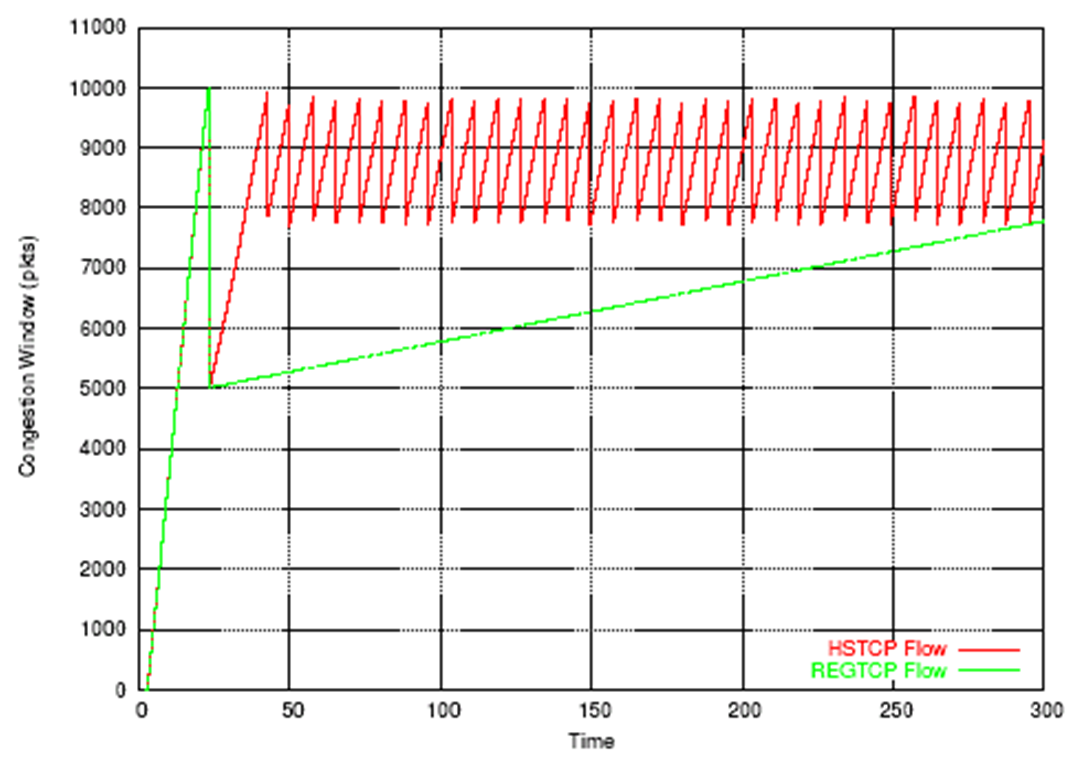
\includegraphics[width=0.9\textwidth]{figures/HSTCP.png}
    \caption{Dynamics of HighSpeedTCP (HSTCP) vs. TCP Reno (REGTCP)}
    \label{fig:HSvsReno}
\end{figure}

Another early implementation is \textbf{Scalable TCP}~\cite{ScalableTCP} where scalability is provided through
\textbf{MIMD} mechanism. In this variant the Congestion Avoidance phase  -- that determines the long term behavior --
utilizes a multiplicative increase similarly to Slow Start algorithm (with less aggressive parameters) instead of the
conventional additive increase. The future application of Scalable TCP is questionable due to severe problems with
fairness properties~\cite{TCPFairnessAnalysis}. The congestion window control can be formulated as:

\begin{tabular}{ll}
    per-ACK: & $\texttt{cwnd} \leftarrow \texttt{cwnd} + a$       \\
    loss:    & $\texttt{w} \leftarrow \texttt{w} - b \texttt{w}$  \\
\end{tabular}

The creators of the protocol suggest the values $\texttt{a}=0.001$ and $\texttt{b}=0.125$~\cite{ScalableTCP}. The main
differences between TCP Reno and Scalable TCP are shown on Figure~\ref{fig:ScalableVSReno}.

\begin{figure}[H]
    \centering
    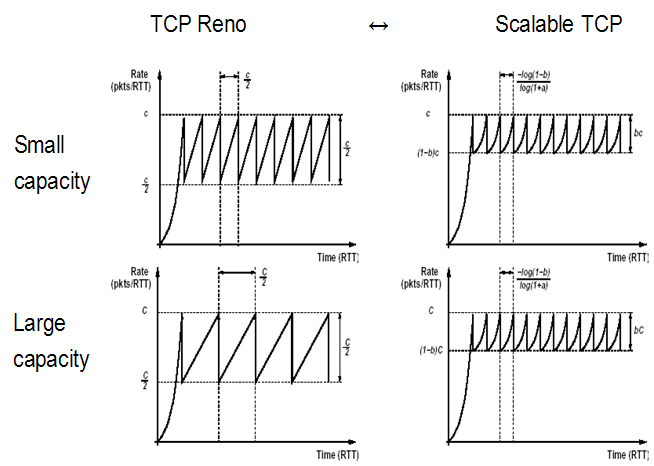
\includegraphics[width=0.9\textwidth]{figures/ScalableTCP.png}
    \caption{Comparison of Scalable TCP and TCP Reno}
    \label{fig:ScalableVSReno}
\end{figure}

The conventional AIMD can not provide fair operation in case when flows have significantly different round trip time.
This so-called RTT unfairness problem is addressed by \textbf{BIC TCP}~\cite{BICTCP} and its successor
\textbf{CUBIC}~\cite{CUBIC}. The BIC TCP utilizes a combination of an additive increase and a binary search based
method with other procedures increasing fairness. CUBIC aims for providing same operating characteristics using way
simple control mechanism where the congestion window is controlled using a cubic function in contrast with the
previously utilized linear, logarithmic and exponential sections. It is worth to note the starting from version 2.6.8
Linux kernel uses BIC TCP as default while starting from 2.6.19 CUBIC is the default TCP implementation. Currently
CUBIC is the default TCP implementation of Linux based systems therefore it has a significant role in today's network
traffic.

Figure~\ref{fig:bictcp} illustrates a period of BIC TCP congestion window adjustment phases. The curve seen on this
figure is hard to express in analytical form and CUBIC approximate this using cubic polynomial functions that results
in similarly good operation characteristics.

\begin{figure}[H]
    \centering
    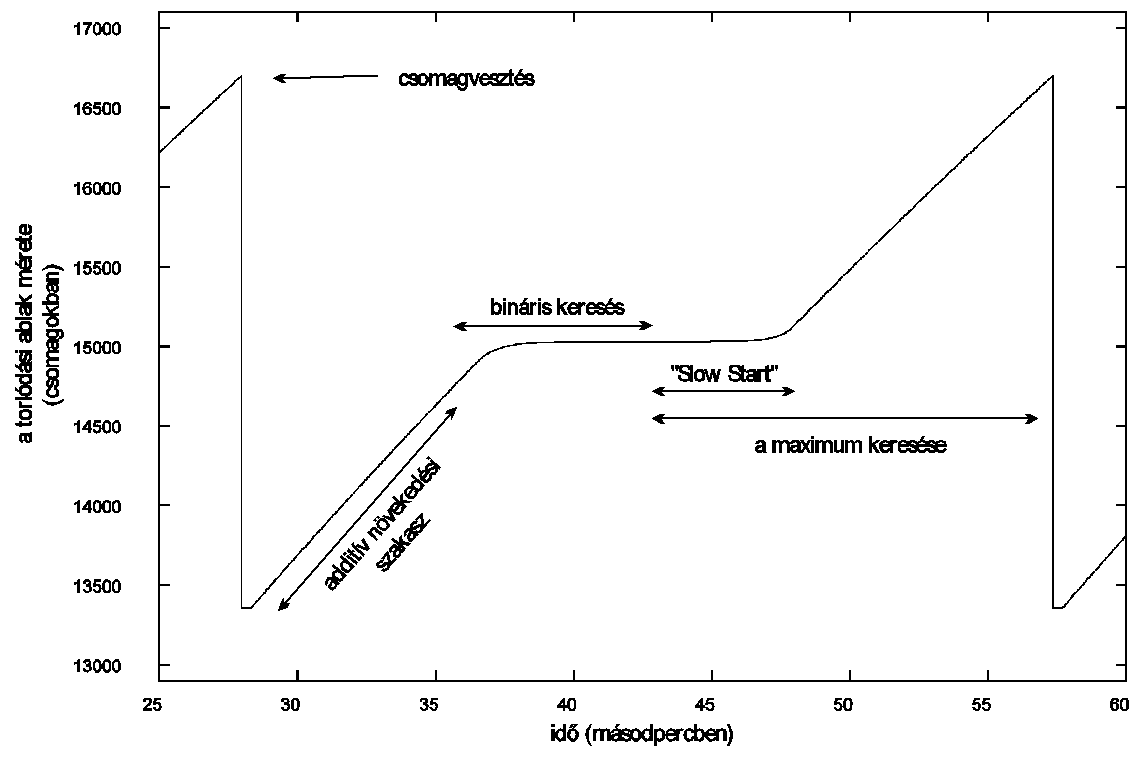
\includegraphics[width=0.9\textwidth]{figures/BICTCP.png}
    \caption{A period of BIC TCP congestion window adjustment}
    \label{fig:bictcp}
\end{figure}

There has been significant proceedings in delay-based congestion control with several protocol recommendations.
Delay-based control first appeared in TCP Vegas protocol. This has been superseded by \textbf{FAST TCP}~\cite{FastTCP}
that is a modified version of TCP Vegas adapted to high speed environments. THe control happens based on the previously
described principles. The protocol tries to keep the number of queued packets between two configured boundary values.
Selecting and tuning these boundary values are not an easy task. FAST TCP protocol with appropriate settings shows
promising results in terms of both network utilization and fairness~\cite{TCPFairnessAnalysis}. The operation
characteristics --that are fundamentally different compared to the previously introduced ones-- are shown on
Figure~\ref{fig:FastTCP}. This has been created using a network setting where one FAST TCP flow is forwarded on the
bottleneck link and the dynamics of the queue and the FAST TCP congestion window size have been captured. It's clearly
visible that after a transient phase the congestion window size stabilizes on a constant value that is able to keep
the queue utilization approximately constant. This eliminates the unwanted oscillation.

\begin{figure}[H]
    \centering
    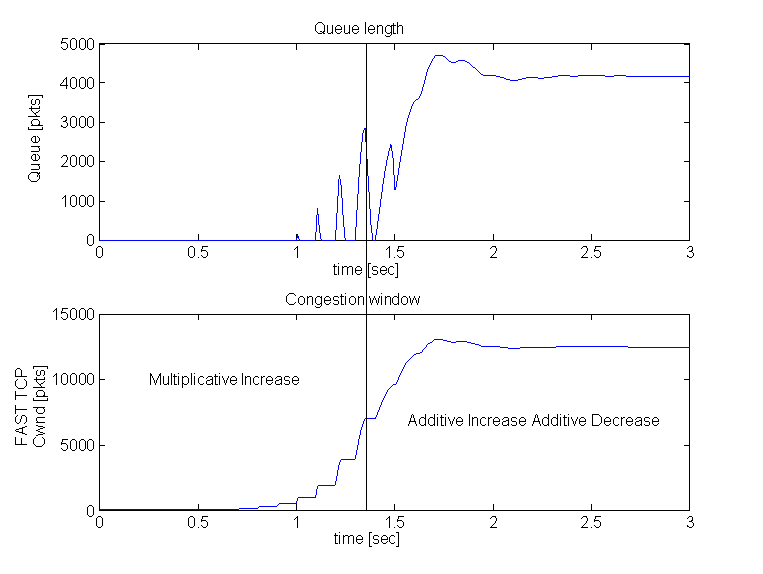
\includegraphics[width=0.9\textwidth]{figures/FAST.png}
    \caption{FAST TCP dynamics}
    \label{fig:FastTCP}
\end{figure}

The current TCP recommendations combine the packet loss and delay-based principles based on various algorithms. Several
methods have been published and implemented out of which the most notable is \textbf{Compound TCP}~\cite{CompundTCP}.
This version has been developed by Microsoft Research employees and is used as a default implementation in Windows
Vista and Windows Server 2008 OSs. Furthermore it is available as a hotfix for other Windows version and also a Linux
based implementation has been created as well. The essence of the protocol that it keeps two congestion window state
variables: a conventional AIMD controlled one and another delay-based controlled. The current size of the congestion
window is the sum of these two components. Based on different network conditions the protocol controls the two
variables using different methods in a way that the resulting behavior provides efficient network utilization and fair
inter-operation with conventional TCP protocol implementations.

\textbf{TCP Westwood}~\cite{TCPWestwood} is one of the TCP implementations with bandwidth approximation based
congestion control that has several variants available. Several approximation procedures have been developed,
implemented and tested over the years that were incorporated in different variants of the protocol.

Finally it has to be noted that there is \textbf{XCP}~\cite{XCP} that is based on explicit signaling of congestion and
therefore requires modified network architecture. In this variant the routers notify the transmitter explicitly about
the level of congestion and can also signal the available bandwidth. In this method the control of utilization and
fairness can be separated clearly. A significant drawback of the protocol is that it requires modification of the
network routers.

One can not foretell that which will be the dominant high speed TCP variant out of the few existing implementations
presented here. Currently this is an active field of research and development in many dominant research facilities all
over the globe. Even comparison of the recommendations is non-trivial since there are no standardized aspects, metrics,
network environments and measurements methods that can provide adequate answers on which protocol is the best or
optimal under given conditions.

\section{Introduction to Network Simulator}

\subsection{Introduction}

\emph{Network Simulator} is a discrete, event-driven, packet based network simulator that is supported by many
universities and research institutes and also it is open-source (\url{http://www.isi.edu/nsnam}). Using this program
beside many things it is possible to inspect routing protocols, multicast and TCP protocols even using wireless
networks.

\textbf{ns} was developed in C++ and otcl languages. The core of the simulator, the protocol implementations and the
computation intensive code was written in C++. In contrast octl script language was used for providing the simulation
configuration and for solutions of one-time tasks that do not require performance.

The class hierarchy of the system is well designed. New functionality can be easily added in C++ to the existing
system, but that is out of scope on this lab. The aim of this class to get a grip on the basics of the otcl interface
and to discover some simple network simulation based measurement methods.

The ns program can be viewed as a tcl interpreter with object-oriented extensions from where the class hierarchy that
supports network simulation is reachable.

As a first step of the simulation an (o)tcl script has to be created that defines the network components, the
interconnection between those components furthermore the timing of the scripted events (e.g. the transmission start
time of a data source). The ns program has to be launched with the script as argument (e.g. \textbf{ns program.tcl})
that produces the log entries and simulation results in output files. During post-processing the simulation result can
be processed using \textbf{awk,perl,gnuplot,excel,etc.} programs. For visual inspection of the results \textbf{nam}
program can be used (NAM - Network Animator) can be used with a log file in special format. This program graphically
visualizes the route of certain packets in the network.

\subsection{Further Reading}\label{sec:tcl}
\begin{itemize}
    \item \href{https://www.tcl.tk/man/tcl8.5/tutorial/tcltutorial.html}{TCL Tutorial}
    \item \href{https://www.isi.edu/nsnam/otcl/doc/tutorial.html}{OTcl tutorial}
    \item \href{http://www.isi.edu/nsnam/ns/ns-documentation.html}{ns manual}
    \item \href{http://alpha.tmit.bme.hu/meresek/tcl2.pdf}{TCL command reference}
\end{itemize}

\subsection{Tcl basics}

Tcl provides rapid prototyping in ns system. In this section a brief overview of the language is given that provides
adequate level of knowledge for completing these measurements.

Commands of a Tcl scipt are separated either by a semi-colon or by a new line. Commands are made of one or more words
where the firs word is the name of the command and optionally the following words are arguments to the command. Words
are separated by space or tab characters.

When evaluating a command the interpreter breaks the commands into words and performs potential replacements then
executes the command with the given arguments. \verb!$variable! is replaced by the value of the variable while
\verb!command! is replaced by the return value of the command. Variables don't have type all value is stored as
string.

Please read the Tcl related materials under Section~\ref{sec:tcl} that are required for successful completion of the
measurements. The program fragment in listing~\ref{lst:10faktorial} calculating the factorial value of 10 contains some
basic language constructs of Tcl.

\begin{lstlisting}[
language=tcl,
captionpos=b,
caption={Tcl program calculating the value of 10!},
label={lst:10faktorial}]
  1:  set fact 1
  2:  for {set i 1} {$i <= 10} {incr i} {
  3:      set fact [expr $fact*$i]
  4:  }
  5:  puts $fact
\end{lstlisting}

In the first line variable \verb!fact! is given the value 1 using the \verb!set!. In the second
line a for loop is started similarly to the C programming language where the braces prevent substitution while
decomposing the command into words. The use of square brackets are illustrated on line 3 where the
\verb!expr! calculates a numeric value and the result of the expression will be stored in the new value of
\verb!fact! -- after executing the \verb!set! command. Finally the result is written to the
output using the \verb!puts! command on the last line.

A recursive way of calculating factorial is show in program listing~\ref{lst:factorial}.

\begin{lstlisting}[
language=tcl,
captionpos=b,
caption={Tcl program for calculating the factorial value of a number},
label={lst:factorial},
showstringspaces=false]
  0:  proc factorial num {
  1:      if {$num > 0} {
  2:          return [expr $num*[factorial [expr $num-1]]]
  3:      } else {
  4:          return 1
  5:      }
  6:  }
  7:  puts [factorial 10]
\end{lstlisting}

\subsection{Otcl basics}

This section introduces the usage of otcl that is an object oriented extension of Tcl language. While an average
\emph{ns} user doesn't have to write new classes it is still beneficial to understand the language constructs of octl.
A classical example found on ns homepage is shown in listing~\ref{lst:nsexample}

\begin{lstlisting}[
language=tcl,
captionpos=b,
caption={Otcl example},
label={lst:nsexample},
showstringspaces=false]
  0:  Class mom
  1:  mom instproc greet {} {
  2:      $self instvar age_
  3:      puts "$age_ year old mom say: How are you doing?"
  4:  }

  5:  Class kid -superclass mom
  6:  kid instproc greet {} {
  7:      $self instvar age_
  8:      puts "$age_ year old kid say: What's up, dude?"
  9:  }

  10:  set a [new mom]
  11:  $a set age_ 45
  12:  set b [new kid]
  13:  $b set age_ 15

  14:  $a greet
  15:  $b greet
\end{lstlisting}

The example in listing~\ref{lst:nsexample} defines class \verb!mom! using the \verb!Class! in
the line 0 that will be the superclass of the class \verb!kid! defined on line 5 using the
\verb!-superclass! keyword. The class definitions are followed by method definitions using the
\verb!instproc! keyword. In lines 2 and 7 the role of \verb!$self! is equivalent with the role of
\verb!this! keyword in C++ language. The \verb!instvar! keyword declares a member variable -- if
that has not been declared before -- furthermore it brings the variable into the scope so it can be referred as a
variable. Finally the \verb!new! command can be used for creating an instance of a class (lines 10 and
12). On line 14 and 15 the methods are invoked producing the following output:
\begin{lstlisting}[language=bash]
45 year old mom say: How are you doing?
15 year old kid say: What's up, dude?
\end{lstlisting}

\section{Simulation program example}

This section demonstrates a simple simulation script described line-by-line showing the basic steps for preparing a
simulation.

The simulated network -- as shown on Figure~\ref{fig:simplesim} -- consists 4 nodes (\verb!n0,n1,n2,n3!). The
duplex link capacity between nodes \verb!n0! \verb!n2! and \verb!n1! and
\verb!n2! is 2Mbps and its delay is 10 milliseconds. The third link between \verb!n2! and
\verb!n3! has a capacity of 1.7 Mbps with a delay of 20 milliseconds. Each node utilizes a 10 packets
capacity \verb!DropTail! mode queue that serves the queued packets in a FIFO manner and drops all incoming
packets if its buffer that is able to hold 10 packets is full.

The TCP agent attached to \verb!n0! node establishes a connection with a TCP \verb!sink!
attached to \verb!n3!. A TCP agent -- by default -- is only capable of generating packets with size of 1
kbyte. The responsibility of the sink is to send back ACKs.

The UDP agent attached to node \verb!n1! is communicating with the \verb!null! agent attached
to node \verb!n3!. The \verb!null! agent is just only frees up the packet associated memory
since UDP does not require sending ACKs back. The \verb!tcp! agent has an attached \verb!ftp!
traffic generator while the \verb!udp! has a \verb!cbr!. The latter is a Constant Bit Rate
data stream generator: it is sending 1 kbyte packtes with 1 Mbps speed. The \verb!cbr! generator operates
between 0.1s and 4.5s while the \verb!ftp! generator operates between 1.0s and 4.0s.

\begin{figure}[H]
    \centering
    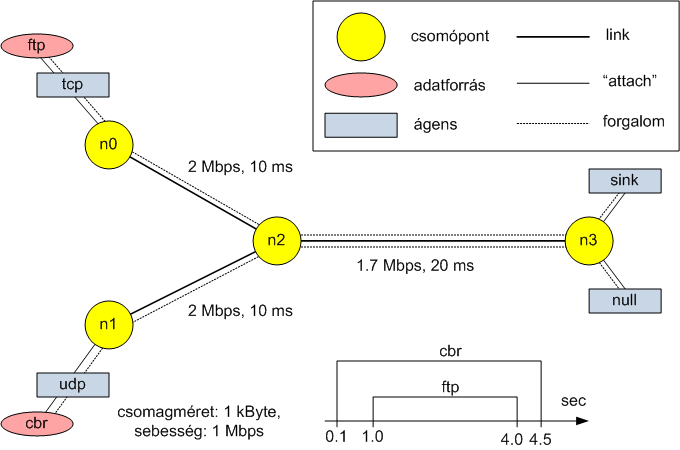
\includegraphics[width=0.9\textwidth]{figures/topology-new.png}
    \caption{Simple topology used for simulation}
    \label{fig:simplesim}
\end{figure}

The simulation topology shown of Figure~\ref{fig:simplesim} is realized by the program in listing~\ref{lst:simexample}.
The explanation of the program follows:

\begin{itemize}

    \item \verb!0: set ns [new Simulator]!: instantiates the ns simulator object and stores it in variable named
          \verb!ns!. This is the opening line of all ns scripts that among other things initializes the
          discrete
          time scheduler. The class \verb!Simulator! has methods for doing the following things:

          \begin{itemize}
              \item create network objects (nodes,links,etc.)
              \item interconnect network objects (e.g. \verb!attach-agent!)
              \item set parameters of network objects
              \item define data link between agents (e.g. between \verb!tcp! and \verb!sink!)
              \item control the presentation parameters of NAM
          \end{itemize}

    \item \verb!1-2: $ns color fid color!: sets the color of the flow identified by flow id \emph{fid}. This setting of the
          \verb!Simulator! object only affects the NAM presentation and does not affect the simulation.

    \item \verb!4: $ns namtrace-all file-descriptor!: enables simulation trace to be saved in NAM format. Similar to
          \verb!trace-all!
          method which dumps data in more general format.

    \item \verb!5: proc finish {}!: this command is executed at the end of the simulation as a result of registering it
          at
          line 52: \verb!$ns at 5.0 "finish"!. After closing the log NAM program is executed as an epilogue of the
          simulation
          script.

    \item \verb!12-15: set n0 [$ns node]!: this method can be used for creating a network node

    \item \verb!16-18: $ns duplex-link <node1> <node2> <capacity> <delay> <queue type>!: creates two simplex links with the given bandwidth and delay and connects the two
          nodes
          with those. Ns specialty is that the output queue is implemented as a part of the link so the queue type has
          to be
          specified when creating a link. If we'd like to use the active queue management \verb!RED!
          instead of
          \verb!DropTail! simply specify that as last argument of the command. Important to note that it's
          possible to
          simulate erroneous links. (please consult the ns documentation for more information)

    \item \verb!20-23!: these commands are relevant for NAM presentation. It's worth examining the output
          after
          commenting out these lines.

\end{itemize}

The part above defines the network topology. The next steps are to attach the traffic agents (TCP,UDP) and configure
the data sources (FTP,CBR) and interconnect every desired component.

\begin{itemize}%[resume]

    \item \verb!24,27,34,36: set tcp [new Agent/TCP]!: This is how a TCP agent can be instantiated. Similarly to this any kind of agent or
          traffic generator can be instantiated if the class name is known. The supported class names are listed in the
          ns
          documentation or alternatively it can be read out from the \verb!ns-2/tcl/libs/ns-default.tcl! file. This file contains
          the default
          parameters of the ns supported network objects. After reading this file one will know what are the supported
          classes
          and which are the configurable parameters of those.

    \item \verb!26,28,35,37: $ns attach-agent <node> <agent>!: This method of the \verb!Simulator! class attaches an agent to a node. The
          \verb!attach-agent! just calls the given node's \verb!attach! method that binds the given agent
          to
          itself. This can be equivalently written as \verb!<node> attach <agent>!.

    \item \verb!29,38: $ns connect <agent1> <agent2>!: after creating agents the logical connection has to be created between them. This
          command can be used for that purpose that sets the corresponding neighboring node's network and port address.

\end{itemize}

After specifying the network configuration the simulation script has to be given i.e. the timing of predefined events
must be specified. The \verb!Simulator! class has several methods related to timing. The most commonly used one
is:

\begin{itemize}

    \item \verb!46-52: $ns at <time> <command>!: The \verb!Simulator! object executes the given command at the given
          simulation
          time-point  using its scheduler. For example line 46. schedules the \verb!start! method of the
          \verb!$cbr! object to be executed at 0.1s that will start traffic generation as a result of that.

\end{itemize}

After settling the topology and timings and registering the end of simulation procedure the last step is to start the
simulation using the command \verb!$ns run!. on line 55.

\begin{lstlisting}[
language=tcl,
captionpos=b,
caption={Simple simulation script},
label={lst:simexample},
showstringspaces=false]
  0:  set ns [new Simulator]  

   1:  $ns color 1 Blue  
   2:  $ns color 2 Red

   3:  set nf [open out.nam w]
   4:  $ns namtrace-all $nf

   5:  proc finish {} {
   6:      global ns nf
   7:      $ns flush-trace
   8:      close $nf  
   9:      exec nam out.nam &
  10:      exit 0
  11:  }

  12:  set n0 [$ns node]
  13:  set n1 [$ns node]
  14:  set n2 [$ns node]
  15:  set n3 [$ns node]

  16:  $ns duplex-link $n0 $n2 2Mb 10ms DropTail
  17:  $ns duplex-link $n1 $n2 2Mb 10ms DropTail
  18:  $ns duplex-link $n2 $n3 1.7Mb 20ms DropTail
  19:  $ns queue-limit $n2 $n3 10

  20:  $ns duplex-link-op $n0 $n2 orient right-down
  21:  $ns duplex-link-op $n1 $n2 orient right-up
  22:  $ns duplex-link-op $n2 $n3 orient right
  23:  $ns duplex-link-op $n2 $n3 queuePos 0.5

  24:  set tcp [new Agent/TCP]
  25:  $tcp set class_ 2
  26:  $ns attach-agent $n0 $tcp
  27:  set sink [new Agent/TCPSink]
  28:  $ns attach-agent $n3 $sink
  29:  $ns connect $tcp $sink
  30:  $tcp set fid_ 1

  31:  set ftp [new Application/FTP]
  32:  $ftp attach-agent $tcp
  33:  $ftp set type_ FTP

  34:  set udp [new Agent/UDP]
  35:  $ns attach-agent $n1 $udp
  36:  set null [new Agent/Null]
  37:  $ns attach-agent $n3 $null
  38:  $ns connect $udp $null
  39:  $udp set fid_ 2

  40:  set cbr [new Application/Traffic/CBR]
  41:  $cbr attach-agent $udp
  42:  $cbr set type_ CBR
  43:  $cbr set packet_size_ 1000
  44:  $cbr set rate_ 1mb
  45:  $cbr set random_ false

  46:  $ns at 0.1 "$cbr start"
  47:  $ns at 1.0 "$ftp start"
  48:  $ns at 4.0 "$ftp stop"
  49:  $ns at 4.5 "$cbr stop"

  50:  $ns at 4.5 "$ns detach-agent $n0 $tcp ;
  51:              $ns detach-agent $n3 $sink"

  52:  $ns at 5.0 "finish"

  53:  puts "CBR packet size = [$cbr set packet_size_]"
  54:  puts "CBR interval = [$cbr set interval_]"

  55:  $ns run
\end{lstlisting}

\subsection{Processing results}

Beside NAM visualization of the simulation results the system provides facilities for creating a log file of all events
of all packet. The \verb!Simulator trace-all! -- in the example the \verb!namtrace-all! was used that produces
different outputs -- method creates an output file whom lines correspond to packet events and is made of 12 space
separated field:
\begin{enumerate}

    \item The type of the event:
          \begin{itemize}
              \item ``r" (receive): the destination node received the packet
              \item ``d" (drop): the packet has been discarded by a queue
              \item ``+" (enqueue): the packet has been enqueued
              \item ``-" (dequeue): the packet has been dequeued
          \end{itemize}

    \item the timestamp of the event (in seconds)

    \item the identifier of the originator node

    \item the identifier of the destination node. This and the originator node determines on which link the event
          happened
          (don't mix-up with the field in 9. and 10.)

    \item The type of the packet

    \item Signaling bits (currently just the ECN bit is used)

    \item Flow id in case of IPv6 that can be set from tcl (see line 30. and 39 in listing~\ref{lst:simexample}); even
          if
          the simulator is not using this id it can be used for evaluating the simulation results or tracing. (e.g. NAM
          uses
          flow-id for coloring purposes)

    \item Source address in \emph{node.port} format

    \item Destination address in \emph{node.port} format

    \item The sequence number of the network protocol; Even if UDP does not use sequence number, ns track these packets
          as
          well for easier tracing

    \item unique ID of the packet

\end{enumerate}

In case of lengthier simulation run when only some aggregated metrics are in the focus of interest it is resource
consuming to log all packet events. NS provides facilities for monitoring a single queue. Details can be found under
the section ``Trace and Monitoring Support" in the ns documentation.

In ns terminology the per packet inspection is referred as ``trace" while the aggregated state inspection is referred
as ``monitoring". The latter is a better candidate to be used in a long term simulation since tracing millions of
millions of packets slows down the simulation while producing enormous -- potentially unmanageable -- output trace
file. As an example one can experiment with a simulation with and without NAM tracing.

Due to performance considerations it is advised to use monitoring. The monitoring related classes are documented in the
above mentioned section in the ns documentation. A simple example is presented in listing~\ref{lst:monitoring} that
extends the previously demonstrated script on how to extend int with by getting a bandwidth utilization graph for link
2-3 with 2 seconds measurement interval. The output file ``2-3.bw" can be plotted by either \verb!xgraph! or
\verb!gnuplot!.

\begin{lstlisting}[
language=tcl,
captionpos=b,
caption={Monitoring extension},
label={lst:monitoring},
showstringspaces=false]
    ...
    set bwSampleInterval 2.0\\
    ...
    [[$ns link $n2 $n3] attach-monitors [new SnoopQueue/In]
        [new SnoopQueue/Out] [new SnoopQueue/Drop] [new QueueMonitor]
    ...
    proc SampleBW {link} {
        global ns bwSampleInterval
        set qm [$link set qMonitor_]
        puts "[$ns now] [expr [$qm set bdepartures_] / $bwSampleInterval]"
        $qm set bdepartures_ 0
        $ns after $bwSampleInterval "SampleBW $link"
    }
    ...
    $ns at 0.0 "SampleBW [$ns link $n2 $n3]"
\end{lstlisting}

\section{Simulation of High-Speed TCP implementations}

Some of the TCP implementation is in file \verb!tcp/tcp.cc! where the \verb!opencwnd! and the
\verb!slowdown! functions should be studied for setting the right value for the desired version (see
wnd\_option\_ in the C++ source and windowOption\_ in tcl).
Some other portion of the TCP implementations are in separate files and classes (see FAST TCP in
\verb!tcp-fast.cc!).

When simulating newer TCP versions it's better to not use the basic TCP agent but the SACK option instead. The sending
and receiving agents can be instantiated with these commands:

\begin{lstlisting}[
language=tcl,
captionpos=b,
caption={Using SACK instead of basic agent},
label={lst:sackagent},
showstringspaces=false]
    set tcp [new Agent/TCP/Sack1]
    set sink [new Agent/TCPSink/Sack1]
\end{lstlisting}

Selecting the appropriate TCP agent happens by setting the TCP agent's \verb!windowOption_! member variable:

\begin{lstlisting}[
language=tcl,
captionpos=b,
caption={Setting the TCP agent's window option},
label={lst:windowoption},
showstringspaces=false]
    $tcp set windowOption_ 8
\end{lstlisting}

The ns-2 version used during this lab has the following TCP versions:

\begin{tabular}{|l|l|}
    \hline
    \cellcolor{blue!25} \textbf{protocol} & \cellcolor{blue!25} \textbf{windowOption\_}  \\\hline
    HighSpeed TCP                         & 8                                            \\\hline
    Scalable TCP                          & 9                                            \\\hline
    BIC TCP                               & 12                                           \\\hline
    CUBIC                                 & 13                                           \\\hline
\end{tabular}

\hfill \break
FAST TCP objects has to be instantiated from the appropriate classes (the receiver stays the same):

\begin{lstlisting}[
language=tcl,
captionpos=b,
caption={Fast TCP instantiation},
label={lst:fasttcp},
showstringspaces=false]
    set fasttcp [new Agent/TCP/Fast]
    set sink [new Agent/TCPSink/Sack1]
\end{lstlisting}

\bibliographystyle{unsrt}
\bibliography{references}

\appendix

\section{Entry quiz sample questions}

\begin{enumerate}
    \item What are the operational phases of conventional TCP Reno protocol?
    \item What happens in the Slow Start phase?
    \item Describe the essence of AIMD mechanism.
    \item What types of congestion control principles do you aware of?
    \item Enumerate at least 3 high-speed, packet loss based TCP version.
    \item How do the delay-based TCP versions operate? What are the differences compared to conventional TCP?
    \item What type of congestion control mechanism does Scalable TCP utilize?
\end{enumerate}

\section{Lab exercises}

\subsection{Lab environment}

The lab PCs have Network Simulator 2.33 installed. The source code can be found
under /home/user/ns-allinone-2.33/ns-2.33 directory and the executable location is also
appended to \verb!$PATH! variable.
A simulation can be started e.g. from a directory named \verb!tcp-measurement! under home directory
by simply executing:

\begin{lstlisting}[language=bash]
ns sim.tcl [param1 param2 ...]
\end{lstlisting}

\subsection{Preparation}

Study the handed out scripts :
\href{https://qosip.tmit.bme.hu/foswiki/pub/Meres/NagysebesseguTCPSzimulaciokFeladatok/sim.tcl}{sim.tcl}
and \href{https://qosip.tmit.bme.hu/foswiki/pub/Meres/NagysebesseguTCPSzimulaciokFeladatok/utils.tcl}{utils.tcl}.
\verb!utils.tcl! contains utility functions that can be used during this lab after customizing them.
\verb!sim.tcl! is the skeleton of the main simulation script. During the measurements this script
has to be extended according to the concrete tasks.

The outputs of the simulations are text files that for example can contain the dynamics of
the congestion window. E.g. every 0.01 seconds a line is appended to the output file containing
two fields where the first field is the timestamp and the second field is the size of the congestion
window expressed in number of packet size. These output files have to be evaluated. For visualization either
\href{http://www.xgraph.org/}{xgraph}
or \href{http://www.gnuplot.info/}{gnuplot} can be used.

A lab report has to be created that documents the source codes created during this lab and also contains the
figures and evaluation results.

\subsection{Standalone TCP flows on a simple topology}

Create a simple topology that contains 2 network nodes and 1 link (``dumb-bell topology").
Set the link speed to 1 GBps with one way delay of 50 ms. Set the queue size of the link to 8300 packets with packet
size of 1460 bytes (1500 bytes including headers).
(Use 100Mbps link with 5 ms delay and  83 packets queue for testing the basic operation.)
Evaluate the operation of standalone TCP flow operation with different TCP implementations -- standalone here means
that there is only one flow in the network
doing unlimited FTP download. T
The available TCP implementations are: HighSpeed TCP, Scalable TCP, BIC TCP, CUBIC, FAST TCP. Out of these carry-out
evaluation of at least \textbf{one} packet loss based and \textbf{one} delay-based protocol.
During the measurement record the dynamics of the TCP flow congestion window size (cwnd) and the bandwidth(throughput)
and
the queue depth of the link.

\textbf{Hint:} \hfill \break

To monitor the queue depth a queue monitor object has to be used that can be created using the following code:

\begin{lstlisting}[
language=tcl,
showstringspaces=false]
    set qmon [$ns monitor-queue $n1 $n2 ""]
    print-queue $queue_measurement_interval $qfp
\end{lstlisting}

This will result in monitoring the queue depth in every queue measurement interval. (Check the procedure's code in
\verb!utils.tcl! file!)

For monitoring different flows a flow monitor object has to be used that can monitor the behavior of individual flows
based on the appropriate IDs.
A flow monitor can be created like:

\begin{lstlisting}[
language=tcl,
showstringspaces=false]
    set fmon [$ns makeflowmon Fid]
    $ns attach-fmon [$ns link $n1 $n2] $fmon
\end{lstlisting}

In order to record TCP flows congestion windows and throughput the \verb!print-cwnd! and \verb!print-thput!
procedures can be used(see \verb!utils.tcl!).
Notice that in case of	\verb!print-cwnd! the source TCP agent has to be specified while in case of
\verb!print-thput! the flow ID has to be given!.
For measuring the throughput of a flow the counters have to be reset by using the \verb!lastKBytes($flow_id)! command.

A useful helper procedure is \verb!timeackReport! that can be used for periodic feedback on
the transmission progress status of each flow.

\subsection{Evaluating TCP flow contention on a simple topology}

\subsubsection{Packet loss based variants}\label{sec:plossexercise}

Using the previously created topology examine the behavior of operating two different packet loss based
TCP implementation side-by-side. Examine the effects of starting the different flows at different time points.
What happens in that case? What is the level of fairness between the two choses TCP implementation?

\subsubsection{Packet loss and delay-based variants}

Carry out similar measurement as before in~\ref{sec:plossexercise} but now using an arbitrarily chosen
packet loss based protocol and FAST TCP side-by-side. Evaluate the effects of FAST TCP's alpha and beta parameters on
fairness.

\end{document}